% =============================================================================
%  week15_diffusion.tex
%  Diffusion Models: From VAEs to DDPM — Full Mathematical Derivation
%  Morten Hjorth-Jensen, May 2026
%  Revised: code slides removed; VAE kept as motivation; new derivations added
% =============================================================================

\documentclass[aspectratio=169,11pt]{beamer}

\usetheme{Madrid}
\usecolortheme{default}
\usefonttheme[onlymath]{serif}

\setbeamercolor{frametitle}{bg=blue!11!white, fg=blue!60!white}
\setbeamercolor{title}{fg=blue!65!white}
\setbeamercolor{block title}{bg=blue!16!white, fg=blue!60!white}
\setbeamercolor{block body}{bg=blue!4!white}
\setbeamercolor{alerted text}{fg=red!65!black}
\setbeamertemplate{navigation symbols}{}
\setbeamertemplate{footline}{%
  \leavevmode\hbox{%
    \begin{beamercolorbox}[wd=.30\paperwidth,ht=2.25ex,dp=1ex,center]{author in head/foot}%
      \usebeamerfont{author in head/foot}\insertshortauthor
    \end{beamercolorbox}%
    \begin{beamercolorbox}[wd=.44\paperwidth,ht=2.25ex,dp=1ex,center]{title in head/foot}%
      \usebeamerfont{title in head/foot}\insertshorttitle
    \end{beamercolorbox}%
    \begin{beamercolorbox}[wd=.26\paperwidth,ht=2.25ex,dp=1ex,right]{date in head/foot}%
      \usebeamerfont{date in head/foot}\insertshortdate{}\hspace*{1em}%
      \insertframenumber/\inserttotalframenumber\hspace*{1ex}
    \end{beamercolorbox}}%
  \vskip0pt}

\usepackage[utf8]{inputenc}
\usepackage[T1]{fontenc}
\usepackage{amsmath,amssymb,amsfonts,mathtools,bm}
\usepackage{booktabs}
\usepackage{xcolor}
\usepackage{tikz}
\usetikzlibrary{arrows.meta,positioning,shapes.geometric,decorations.pathreplacing}
\usepackage{hyperref}

% ── Convenience macros ───────────────────────────────────────────────────────
\newcommand{\E}{\mathbb{E}}
\newcommand{\R}{\mathbb{R}}
\newcommand{\DKL}{D_{\mathrm{KL}}}
\newcommand{\Norm}{\mathcal{N}}
\newcommand{\ELBO}{\mathcal{L}}
\newcommand{\bx}{\bm{x}}
\newcommand{\bh}{\bm{h}}
\newcommand{\bz}{\bm{z}}
\newcommand{\beps}{\bm{\epsilon}}
\newcommand{\bmu}{\bm{\mu}}
\newcommand{\bsig}{\bm{\sigma}}
\newcommand{\btheta}{\bm{\theta}}
\newcommand{\bphi}{\bm{\phi}}
\newcommand{\half}{\tfrac{1}{2}}
% ── Additional macros for GAN section ────────────────────────────────────────
\newcommand{\pr}{p_{r}}           % real data distribution
\newcommand{\pg}{p_{g}}           % generator distribution
\newcommand{\pz}{p_{z}}           % noise prior
\newcommand{\JS}{D_{\mathrm{JS}}} % Jensen-Shannon divergence
\newcommand{\KL}{D_{\mathrm{KL}}} % alias matching GAN notation (= \DKL)
\DeclareMathOperator*{\argmax}{arg\,max}
\DeclareMathOperator*{\argmin}{arg\,min}

% ── Metadata ─────────────────────────────────────────────────────────────────
\title[GANs]{Generative Adversarial Networks and Summary of Course}
\subtitle{FYS5429/9429}
\author[M.\ Hjorth-Jensen]{Morten Hjorth-Jensen}
\institute[UiO/MSU]{Department of Physics \& CCSE, University of Oslo}
\date{May 21, 2026}

% =============================================================================
\begin{document}
% =============================================================================

\begin{frame}[plain]
  \titlepage
\end{frame}

% ── Table of contents ─────────────────────────────────────────────────────────
\begin{frame}[allowframebreaks]{Outline}
  \scriptsize
  \tableofcontents[hideallsubsections]
\end{frame}

% =============================================================================
\section{Motivation: VAEs and Their Limits}
% =============================================================================

% -----------------------------------------------------------------------------
\begin{frame}{Generative models: the common thread}

All deep generative models share one goal: learn a distribution
$p_{\btheta}(\bx)$ over data~$\bx$ that we can both evaluate and sample from.

\medskip
\begin{center}
\renewcommand{\arraystretch}{1.25}
\begin{tabular}{llll}
\toprule
\textbf{Family} & \textbf{Latent} & \textbf{Training signal} & \textbf{Sample cost}\\
\midrule
VAE            & $\bh \in \R^{d_h},\;d_h\!\ll\!d_x$ & ELBO             & 1 decoder pass\\
\textbf{Diffusion} & $\bx_t\in\R^{d_x}$ (full dim)  & \textbf{ELBO, $T$ levels} & $T$ denoiser calls\\
GAN            & $\bz\in\R^k$                       & Adversarial      & 1 generator pass\\
\bottomrule
\end{tabular}
\end{center}

\medskip
\begin{alertblock}{Key insight}
Diffusion models are \textbf{hierarchical VAEs} with $T$ latent levels,
a fixed (non-learned) encoder, and full-dimensional latents.
Understanding VAEs is the fastest route to understanding diffusion.
\end{alertblock}
\end{frame}


% =============================================================================
\section{Generative Adversarial Networks}
% =============================================================================

\begin{frame}{Transition: From Likelihood to Adversarial Training}

So far we studied models maximising (a lower bound on) $\log p(\bx)$:

\smallskip
\begin{center}
\renewcommand{\arraystretch}{1.2}
\begin{tabular}{lll}
\toprule
\textbf{Model} & \textbf{Objective} & \textbf{Key idea}\\
\midrule
VAE  & Maximise ELBO          & Variational inference, 1 latent level\\
DDPM & Maximise ELBO ($T$ levels) & Fixed encoder, noise prediction\\
\textbf{GAN}  & \textbf{No likelihood bound} & \textbf{Adversarial game}\\
\bottomrule
\end{tabular}
\end{center}

\smallskip
\begin{alertblock}{Fundamental difference}
GANs never evaluate $\log p_{\btheta}(\bx)$.
A \textbf{discriminator} $D$ provides the training signal by classifying
real vs.\ fake, driving the \textbf{generator} $G$ to match $p_r$ —
without any likelihood computation.\\[2pt]
\textit{Benefit}: sharper samples, no $\ell_2$-blurring.
\quad\textit{Cost}: no likelihood, mode collapse risk, instability.
\end{alertblock}
\end{frame}

\section{What Is a GAN?}
%% ═══════════════════════════════════════════════════════════

\begin{frame}{Generative Adversarial Networks}
  A \textbf{GAN} (Goodfellow et al., NeurIPS 2014) pits two neural
  networks against each other in a zero-sum game:

  \medskip
  \begin{columns}[T]
    \column{0.50\textwidth}
      \begin{block}{Generator $G$}
        \begin{itemize}
          \item Input: noise $\bz\sim\pz(\bz)$
          \item Output: synthetic sample
                $\bx = G(\bz;\btheta^{(g)})$
          \item Goal: fool the discriminator
          \item Implicitly defines distribution $\pg$
        \end{itemize}
      \end{block}
    \column{0.47\textwidth}
      \begin{block}{Discriminator $D$}
        \begin{itemize}
          \item Input: image $\bx$
          \item Output: $D(\bx;\btheta^{(d)})\in(0,1)$
            $=\Pr(\bx\text{ is real})$
          \item Goal: distinguish real from fake
        \end{itemize}
      \end{block}
  \end{columns}

  \bigskip
  \begin{alertblock}{Key insight}
    Neither network sees the other's parameters.
    They improve \emph{each other} through adversarial feedback alone.
  \end{alertblock}
\end{frame}

\begin{frame}{GAN Architecture (Schematic)}
  \begin{center}
  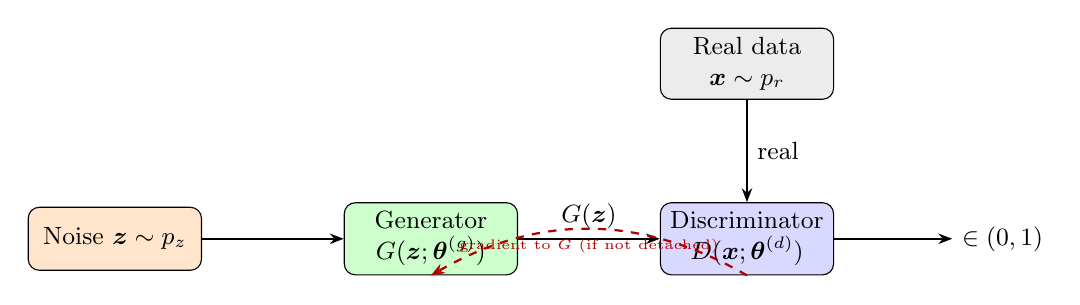
\begin{tikzpicture}[
      node distance=1.3cm and 1.8cm,
      box/.style={draw, rounded corners=4pt, minimum width=2.2cm,
                  minimum height=0.8cm, align=center, font=\small},
      arrow/.style={-{Stealth[length=5pt]}, thick}
    ]
    \node[box, fill=orange!20]  (noise)  {Noise $\bz\sim\pz$};
    \node[box, fill=green!20,   right=of noise] (G) {Generator\\$G(\bz;\btheta^{(g)})$};
    \node[box, fill=blue!15,    right=of G]     (D) {Discriminator\\$D(\bx;\btheta^{(d)})$};
    \node[box, fill=gray!15,    above=of D]     (real) {Real data\\$\bx\sim\pr$};
    \node[right=1.5cm of D, font=\small] (out) {$\in(0,1)$};

    \draw[arrow] (noise) -- (G) node[midway,above,font=\tiny] {};
    \draw[arrow] (G)     -- (D) node[midway,above,font=\small] {$G(\bz)$};
    \draw[arrow] (real)  -- (D) node[midway,right,font=\small] {real};
    \draw[arrow] (D)     -- (out);

    % Gradient arrows back
    \draw[arrow,dashed,red!70!black,bend right=30]
      (D.south) to node[below,font=\tiny,red!70!black]
      {gradient to $G$ (if not detached)} (G.south);
  \end{tikzpicture}
  \end{center}

  \medskip
  \begin{itemize}
    \item $G$ maps $\bz\in\R^k\to\R^d$ (noise $\to$ data space)
    \item $D$ maps $\bx\in\R^d\to(0,1)$ (image $\to$ probability)
    \item Training alternates: freeze $G$ and update $D$; freeze $D$ and update $G$
  \end{itemize}
\end{frame}

\begin{frame}{Learning Paradigms and Applications}
  \begin{columns}[T]
    \column{0.50\textwidth}
      \textbf{Three learning settings:}
      \begin{enumerate}
        \item \textbf{Unsupervised} — no labels; $G$ learns the full data manifold
        \item \textbf{Supervised} — conditional GAN conditions $G$ on class label
        \item \textbf{Semi-supervised} — $D$ doubles as a feature extractor
      \end{enumerate}

    \column{0.47\textwidth}
      \textbf{Applications:}
      \begin{itemize}
        \item Image synthesis / super-resolution
        \item Text-to-image translation
        \item Video prediction
        \item Data augmentation for rare events
        \item Anomaly detection
        \item Scientific simulation:\\
              particle physics, drug discovery,\\
              climate modelling
      \end{itemize}
  \end{columns}
\end{frame}

%% ═══════════════════════════════════════════════════════════
\section{Mathematical Formulation}
%% ═══════════════════════════════════════════════════════════

\begin{frame}{Notation and Probability Spaces}
  \begin{center}
  \renewcommand{\arraystretch}{1.25}
  \begin{tabular}{ll}
    \toprule
    Symbol & Meaning\\
    \midrule
    $\pr(\bx)$ & Real data distribution (unknown; represented by training set)\\
    $\pz(\bz)$ & Latent noise prior, e.g.\ $\mathcal{N}(\mathbf{0},I)$\\
    $G(\bz;\btheta^{(g)})$ & Generator: differentiable map $\R^k\to\R^d$\\
    $\pg$ & Generator distribution = push-forward of $\pz$ through $G$\\
    $D(\bx;\btheta^{(d)})\in(0,1)$ & Discriminator: $\Pr(\bx\text{ is real})$\\
    \bottomrule
  \end{tabular}
  \end{center}

  \medskip
  \textbf{Implicit distribution.} For invertible $G$ the change-of-variables gives:
  \[
    \pg(\bx) = \pz\!\left(G^{-1}(\bx)\right)\,
    \left|\det\frac{\partial G^{-1}}{\partial\bx}\right|.
  \]
  In practice $G$ is not invertible; $\pg$ is an \emph{implicit} distribution
  accessed only through sampling.
\end{frame}

\begin{frame}{The Minimax Objective}
  \begin{block}{Value function (Goodfellow et al., 2014)}
    \[
      \boxed{
        \min_{G}\;\max_{D}\;V(G,D)
        = \underbrace{\E_{\bx\sim\pr}[\log D(\bx)]}_{\text{$D$ correct on real}}
        + \underbrace{\E_{\bz\sim\pz}[\log(1-D(G(\bz)))]}_{\text{$D$ correct on fake}}
      }
    \]
  \end{block}

  \medskip
  \begin{columns}[T]
    \column{0.48\textwidth}
      \textbf{Discriminator (maximise $V$):}
      \begin{itemize}
        \item $D(\bx)\to 1$ on real data
        \item $D(G(\bz))\to 0$ on generated data
      \end{itemize}
    \column{0.48\textwidth}
      \textbf{Generator (minimise $V$):}
      \begin{itemize}
        \item $D(G(\bz))\to 1$ (fool $D$)
        \item $\E_{\pr}[\log D(\bx)]$ is constant w.r.t.\ $G$,
              so $G$ minimises $\E[\log(1-D(G(\bz)))]$
      \end{itemize}
  \end{columns}
\end{frame}

\begin{frame}{Non-Saturating Generator Loss}
  \begin{columns}[T]
    \column{0.52\textwidth}
      \textbf{Problem with the original objective.}
      Early in training $D$ is strong, so $D(G(\bz))\approx 0$:
      \[
        \frac{\partial}{\partial\btheta^{(g)}}\log(1-D(G(\bz)))
        \approx \frac{\partial}{\partial\btheta^{(g)}}\log 1 = 0.
      \]
      The gradient \emph{vanishes} before $G$ has learned anything.

    \column{0.45\textwidth}
      \begin{alertblock}{Fix: non-saturating loss}
        Instead of minimising $\log(1-D(G(\bz)))$,\\
        maximise $\log D(G(\bz))$:
        \[
          \mathcal{L}_G^{\text{non-sat}}
          = -\E_{\bz\sim\pz}[\log D(G(\bz))].
        \]
        Same Nash equilibrium; stronger gradient when $D(G(\bz))\approx 0$.
      \end{alertblock}
  \end{columns}

  \medskip
  \begin{center}
  \renewcommand{\arraystretch}{1.2}
  \begin{tabular}{lcc}
    \toprule
    Loss form & Value at $D(G(\bz))=\varepsilon\approx0$
              & $|\text{gradient}|$\\
    \midrule
    $\log(1-\varepsilon)$ & $\approx-\varepsilon$ & $\approx 1$ (small)\\
    $-\log\varepsilon$    & $+\infty$             & $1/\varepsilon\to\infty$ (large)\\
    \bottomrule
  \end{tabular}
  \end{center}
\end{frame}

\begin{frame}{The Alternating Gradient Algorithm}
  \begin{block}{One training iteration}
    \begin{enumerate}
      \setlength\itemsep{4pt}
      \item \textbf{Freeze $G$}; gradient \textbf{ascent} on $D$:
            \[
              \btheta^{(d)} \leftarrow \btheta^{(d)}
              + \eta\,\nabla_{\btheta^{(d)}}V(G,D).
            \]

      \item \textbf{Freeze $D$}; gradient \textbf{descent} on $G$:
            \[
              \btheta^{(g)} \leftarrow \btheta^{(g)}
              - \eta\,\nabla_{\btheta^{(g)}}\mathcal{L}_G.
            \]
    \end{enumerate}
  \end{block}

  \medskip
  \begin{itemize}
    \item One $D$ step per $G$ step in practice ($k=1$).
    \item Fake images are \textbf{detached} from the computation graph during
          the $D$ step to prevent spurious gradients flowing into $G$.
    \item Both networks update simultaneously — this does \emph{not} guarantee
          convergence (see Section~\ref{sec:challenges}).
  \end{itemize}
\end{frame}

%% ═══════════════════════════════════════════════════════════
\section{Optimal Discriminator and JS Divergence}
%% ═══════════════════════════════════════════════════════════

\begin{frame}{Deriving the Optimal Discriminator}
\small
  Fix $G$ (hence fix $\pg$). Write $V$ as an integral:
  \[
    V(G,D) = \int_{\bx}
    \bigl[\pr(\bx)\log D(\bx) + \pg(\bx)\log(1-D(\bx))\bigr]\,d\bx.
  \]

  \smallskip
  For each $\bx$ independently, maximise the integrand
  $f(t)=A\log t+B\log(1-t)$, $A=\pr(\bx)$, $B=\pg(\bx)$, $t=D(\bx)\in(0,1)$:
  \[
    f'(t) = \frac{A}{t} - \frac{B}{1-t}
    = \frac{A-(A+B)t}{t(1-t)} = 0
    \;\Longrightarrow\; t^* = \frac{A}{A+B}.
  \]

  Check: $f''(t^*) = -A/(t^*)^2 - B/(1-t^*)^2 < 0$ \; $\checkmark$ (maximum).

  \begin{block}{Optimal discriminator}
    \[
      \boxed{D^*(\bx) = \frac{\pr(\bx)}{\pr(\bx)+\pg(\bx)}.}
    \]
    This is the \textbf{Bayes-optimal classifier} for the two-class problem
    \{real, fake\} under equal class priors.
  \end{block}
\end{frame}

\begin{frame}{Nash Equilibrium and Loss at the Optimum}
  \begin{columns}[T]
    \column{0.50\textwidth}
      \textbf{Nash equilibrium.}
      At $\pg=\pr$:
      \[
        D^*(\bx) = \frac{\pr(\bx)}{\pr(\bx)+\pr(\bx)} = \frac{1}{2}.
      \]
      The discriminator cannot distinguish real from fake —
      it is reduced to random guessing.

      \medskip
      \textbf{Loss at the equilibrium.}
      Substituting $D^*=1/2$:
      \begin{align*}
        V(G^*,D^*)
        &= \log\!\tfrac{1}{2}\int\pr\,d\bx
         + \log\!\tfrac{1}{2}\int\pr\,d\bx\\
        &= -2\log 2 \approx -1.386.
      \end{align*}

    \column{0.47\textwidth}
      \begin{alertblock}{Convergence indicator}
        In practice, monitor $D(\bx)$ and $D(G(\bz))$ during training.
        Both should converge to $0.5$ at equilibrium.
        If $D(G(\bz))\ll 0.5$, the generator is losing.
        If $D(\bx)\ll 0.5$, the discriminator is failing.
      \end{alertblock}
  \end{columns}
\end{frame}

\begin{frame}{KL and JS Divergences}
  \textbf{Kullback-Leibler divergence:}
  \[
    \KL(p\|q) = \int p(\bx)\log\frac{p(\bx)}{q(\bx)}\,d\bx
    \;\ge 0,
  \]
  with equality iff $p=q$ a.e.\ (Gibbs' inequality).
  Note: $\KL(p\|q)\ne\KL(q\|p)$ in general.

  \smallskip
  \textbf{Jensen-Shannon divergence} (symmetric, bounded):
  \[
    \JS(p\|q)
    = \frac{1}{2}\KL\!\left(p\,\Big\|\,\frac{p+q}{2}\right)
    + \frac{1}{2}\KL\!\left(q\,\Big\|\,\frac{p+q}{2}\right).
  \]

  \begin{block}{Properties of $\JS$}
    \begin{itemize}
      \item Symmetric: $\JS(p\|q)=\JS(q\|p)$
      \item Non-negative: $\JS(p\|q)\ge 0$, with equality iff $p=q$
      \item Bounded: $\JS(p\|q)\in[0,\log 2]$ for any $p,q$
      \item Related to total variation: $\JS(p\|q)\le\log 2\cdot\mathrm{TV}(p,q)$
    \end{itemize}
  \end{block}
\end{frame}

\begin{frame}{GAN Loss $=$ Jensen-Shannon Divergence}
  Expanding $\JS(\pr\|\pg)$ and simplifying:
  \begin{align*}
    \JS(\pr\|\pg)
    &= \frac{1}{2}\KL\!\left(\pr\,\Big\|\,\frac{\pr+\pg}{2}\right)
     + \frac{1}{2}\KL\!\left(\pg\,\Big\|\,\frac{\pr+\pg}{2}\right)\\
    &= \frac{1}{2}\!\left(\log 2
       + \int\pr\log\frac{\pr}{\pr+\pg}\,d\bx\right)
     + \frac{1}{2}\!\left(\log 2
       + \int\pg\log\frac{\pg}{\pr+\pg}\,d\bx\right).
  \end{align*}

  Recognising $V(G,D^*)$ in the integrals:

  \begin{block}{Main theorem (Goodfellow et al.\ 2014)}
    \[
      \boxed{V(G,D^*) = 2\,\JS(\pr\|\pg) - 2\log 2.}
    \]
    \textbf{Conclusion.} The GAN minimax objective is equivalent to minimising the
    Jensen-Shannon divergence between $\pr$ and $\pg$.
    The global minimum $-2\log 2$ is achieved when $\pg=\pr$.
  \end{block}
\end{frame}

%% ═══════════════════════════════════════════════════════════
\section{Loss Functions in Practice}
%% ═══════════════════════════════════════════════════════════

\begin{frame}{Binary Cross-Entropy Losses}
\small
  \textbf{Discriminator loss} (real label $=s$, fake label $=0$):
  \[
    \mathcal{L}_D
    = -\frac{1}{N}\sum_{i=1}^N \log D(\bx_i)
      -\frac{1}{M}\sum_{j=1}^M \log\bigl(1-D(G(\bz_j))\bigr).
  \]
  \textbf{Generator loss} (non-saturating):
  \[
    \mathcal{L}_G
    = -\frac{1}{M}\sum_{j=1}^M \log D(G(\bz_j)).
  \]
  \begin{block}{One-sided label smoothing ($s=0.9$)}
    Replace real target $1$ with $s<1$. The optimal discriminator becomes
    $D^*_s(\bx) = s\cdot\pr(\bx)/(\pr(\bx)+\pg(\bx))$,
    preventing overconfidence and keeping gradients to $G$ alive.
  \end{block}
\end{frame}

\begin{frame}{Wasserstein Distance (WGAN)}
  \begin{columns}[T]
    \column{0.52\textwidth}
      \small
      \textbf{Problem with JS divergence.}
      When $\pr$ and $\pg$ have non-overlapping supports
      (common early in training): $\JS(\pr\|\pg)=\log 2$ constantly,
      giving zero gradient everywhere.

      \smallskip
      \textbf{Wasserstein-1 distance} (\emph{Earth-mover}):
      \begin{align*}
        W(\pr,\pg) &= \inf_{\gamma\in\Pi(\pr,\pg)}\,
          \E_{(\bx,\mathbf{y})\sim\gamma}\|\bx-\mathbf{y}\|
      \end{align*}
      $\Pi(\pr,\pg)$: all couplings with marginals $\pr$, $\pg$.

    \column{0.43\textwidth}
      \begin{block}{Kantorovich-Rubinstein duality}
        \[
          W(\pr,\pg) = \sup_{\|f\|_L\le 1}
          \bigl(\E_{\pr}[f] - \E_{\pg}[f]\bigr).
        \]
        Sup.\ over all 1-Lipschitz functions $f$.
      \end{block}
      \begin{alertblock}{Advantage}
        $W$ gives meaningful gradients
        even when $\pr\cap\pg=\emptyset$.
        Training is more stable.
      \end{alertblock}
  \end{columns}
\end{frame}

\begin{frame}{WGAN: Gradient Penalty}
  \textbf{WGAN critic.} Replace $D$ with a critic $f_w$ (no sigmoid):
  \[
    \mathcal{L}_{\mathrm{critic}}
    = \E_{\pg}[f_w(\bx)] - \E_{\pr}[f_w(\bx)]
    + \lambda\,\mathcal{L}_{\mathrm{GP}}.
  \]

  \textbf{Gradient penalty} (Gulrajani et al., 2017):
  \[
    \mathcal{L}_{\mathrm{GP}}
    = \E_{\hat{\bx}}\!\Bigl[
        \bigl(\|\nabla_{\hat{\bx}} f_w(\hat{\bx})\|_2 - 1\bigr)^2
      \Bigr],
  \]
  where $\hat{\bx} = \epsilon\bx + (1-\epsilon)G(\bz)$, $\epsilon\sim U[0,1]$
  (uniform on straight lines between real and fake points).

  \medskip
  \begin{itemize}
    \item Enforces the 1-Lipschitz constraint via soft penalisation.
    \item More stable than weight clipping (original WGAN).
    \item $\lambda=10$ is a standard choice.
  \end{itemize}
\end{frame}

%% ═══════════════════════════════════════════════════════════
\section{Training Challenges}
%% ═══════════════════════════════════════════════════════════

\begin{frame}{Vanishing Gradient}
  \textbf{When does it occur?}
  When $D$ is perfect early in training:
  $D(\bx)=1\;\forall\bx\sim\pr$ and $D(G(\bz))=0\;\forall\bz\sim\pz$.

  \medskip
  \textbf{Original $G$ gradient:}
  \[
    \nabla_{\btheta^{(g)}}\,\E[\log(1-D(G(\bz)))]
    \approx \nabla_{\btheta^{(g)}}\,\E[\log 1] = \mathbf{0}.
  \]
  No information flows to $G$.

  \medskip
  \textbf{Non-saturating loss $-\log D(G(\bz))$:}
  \[
    \nabla_{\btheta^{(g)}}\bigl(-\log D(G(\bz))\bigr)
    = -\frac{1}{D(G(\bz))}\nabla_{\btheta^{(g)}}D(G(\bz)).
  \]
  When $D(G(\bz))\approx 0$, the factor $1/D(G(\bz))\to\infty$ amplifies the gradient
  — learning continues.
\end{frame}

\begin{frame}{Mode Collapse}
  \begin{columns}[T]
    \column{0.52\textwidth}
      \textbf{Definition.} The generator maps many different noise vectors
      $\bz$ to the \emph{same} (or very few) output(s):
      \[
        \mathrm{supp}(\pg) \ll \mathrm{supp}(\pr).
      \]
      The JS divergence can still be low on the covered modes,
      so the loss does not detect collapse.

      \medskip
      \textbf{Why it happens.} Given the current discriminator,
      $G$ finds a single ``safe'' output that fools $D$;
      $D$ then adapts, and $G$ shifts to another single output.
      The two networks chase each other indefinitely.

    \column{0.45\textwidth}
      \textbf{Mitigations:}
      \begin{itemize}
        \item \textbf{Minibatch discrimination}: $D$ sees statistics of a
              batch, not individual images — diversity is rewarded.
        \item \textbf{Unrolled GANs}: $G$ optimises against a future $D$,
              preventing short-sighted collapse.
        \item \textbf{Spectral normalisation}: stabilises $D$ by bounding
              its Lipschitz constant.
        \item \textbf{WGAN}: Wasserstein distance measures full distribution
              mismatch, not just modes.
      \end{itemize}
  \end{columns}
\end{frame}

\begin{frame}{Non-Convergence and the Game-Theoretic View}
  GAN training solves a \textbf{two-player non-cooperative game}:
  \[
    G^* = \argmin_G\,\argmax_D\;V(G,D).
  \]

  \medskip
  \textbf{Nash equilibrium} exists at $\pg=\pr$, $D^*\equiv\tfrac{1}{2}$, but:
  \begin{itemize}
    \item Simultaneous gradient updates do \emph{not} guarantee convergence
          to a Nash equilibrium.
    \item The loss landscape of each player changes at every step
          (non-stationary environment).
    \item If $\max_D V(G,D)$ is not convex in $\btheta^{(g)}$,
          global convergence fails even in theory.
  \end{itemize}

  \medskip
  \textbf{Practical stabilisation:}
  \begin{itemize}
    \item Lower $\beta_1$ in Adam (reduces momentum: $0.5$ instead of $0.9$)
    \item One-sided label smoothing
    \item Spectral normalisation of $D$'s weights
    \item Progressive growing (ProGAN), self-attention (SAGAN)
    \item Two-time-scale updates: different learning rates for $G$ and $D$
  \end{itemize}
\end{frame}

%% ═══════════════════════════════════════════════════════════
\section{Evaluating GANs}
%% ═══════════════════════════════════════════════════════════

\begin{frame}{Evaluation Metrics: Overview}
  Evaluating generative models is hard: there is no ground truth output to compare against.

  \medskip
  \begin{center}
  \renewcommand{\arraystretch}{1.25}
  \begin{tabular}{p{2.8cm}p{4.5cm}p{3.5cm}}
    \toprule
    \textbf{Metric} & \textbf{Measures} & \textbf{Limitation}\\
    \midrule
    Inception Score (IS) & Quality + diversity of generated images & Requires pretrained classifier\\
    FID & Distance between real/fake feature distributions & Sensitive to sample size\\
    MMD & Kernel-based distribution distance & Choice of kernel matters\\
    Precision/Recall & Coverage vs.\ fidelity separately & Requires feature extractor\\
    \bottomrule
  \end{tabular}
  \end{center}
\end{frame}

\begin{frame}{Maximum Mean Discrepancy (MMD)}
  \textbf{Definition in RKHS.}  Let $k:\R^d\times\R^d\to\R$ be a kernel.
  The \textbf{MMD} between distributions $p$, $q$ is:
  \[
    \mathrm{MMD}^2(p,q)
    = \E_{\bx,\bx'\sim p}[k(\bx,\bx')]
    - 2\,\E_{\bx\sim p,\,\mathbf{y}\sim q}[k(\bx,\mathbf{y})]
    + \E_{\mathbf{y},\mathbf{y}'\sim q}[k(\mathbf{y},\mathbf{y}')].
  \]

  With the Gaussian kernel $k(\bx,\mathbf{y})=\exp(-\|\bx-\mathbf{y}\|^2/2\sigma^2)$:
  $\mathrm{MMD}=0$ iff $p=q$ (characteristic kernel property).

  \begin{block}{Unbiased empirical estimator}
    Given $n$ real samples $\{\bx_i\}$ and $m$ fake samples $\{\mathbf{y}_j\}$:
    \[
      \widehat{\mathrm{MMD}}^2
      = \frac{1}{n(n-1)}\!\sum_{i\ne j}\!k(\bx_i,\bx_j)
      - \frac{2}{nm}\sum_{i,j}\!k(\bx_i,\mathbf{y}_j)
      + \frac{1}{m(m-1)}\!\sum_{i\ne j}\!k(\mathbf{y}_i,\mathbf{y}_j).
    \]
    Diagonal terms ($i=j$) excluded for unbiasedness.
  \end{block}
\end{frame}

\begin{frame}{Fr\'echet Inception Distance (FID)}
  \textbf{FID} is currently the most widely used GAN metric.

  \medskip
  \textbf{Procedure:}
  \begin{enumerate}
    \item Extract feature vectors from the \textbf{InceptionV3} penultimate layer
          for $n$ real images and $n$ generated images.
    \item Fit Gaussians: $\mathcal{N}(\mu_r, \Sigma_r)$ and $\mathcal{N}(\mu_g, \Sigma_g)$.
    \item Compute the \textbf{Fr\'echet distance}:
  \end{enumerate}
  \[
    \mathrm{FID}
    = \|\mu_r - \mu_g\|^2
      + \mathrm{Tr}\!\Bigl(
          \Sigma_r + \Sigma_g
          - 2(\Sigma_r\Sigma_g)^{1/2}
        \Bigr).
  \]

  \begin{itemize}
    \item Lower FID = better quality and diversity.
    \item State-of-the-art GANs achieve FID $<5$ on MNIST; $<10$ on CIFAR-10.
    \item Sensitive to sample size $n$ — use $\ge 10\,000$ samples.
  \end{itemize}
\end{frame}

%% ═══════════════════════════════════════════════════════════
\section{Architecture Design}
%% ═══════════════════════════════════════════════════════════

\begin{frame}{Generator Architecture for MNIST}
  \textbf{Fully-connected generator} (Goodfellow et al., 2014 style):

  \small
  \[
    \bz\!\in\!\R^{100}
    \xrightarrow{\text{Lin+BN+LReLU}}
    \R^{256}
    \xrightarrow{\text{Lin+BN+LReLU}}
    \R^{512}
    \xrightarrow{\text{Lin+BN+LReLU}}
    \R^{1024}
    \xrightarrow{\text{Lin+Tanh}}
    \R^{784}
  \]
  \normalsize

  \medskip
  \begin{columns}[T]
    \column{0.50\textwidth}
      \textbf{Design choices:}
      \begin{itemize}
        \item \textbf{BatchNorm} after each Linear layer:\\
              normalises activations, allows higher LR,\\
              stabilises gradient flow
        \item \textbf{LeakyReLU(0.2):} prevents dying ReLU;\\
              small gradient for negative inputs
        \item \textbf{Tanh} output: maps to $[-1,1]$, matching\\
              MNIST normalised to $[-1,1]$
        \item Weights: $\mathcal{N}(0,0.02^2)$ (DCGAN convention)
      \end{itemize}

    \column{0.47\textwidth}
      \textbf{Discriminator differences:}
      \begin{itemize}
        \item \textbf{No BatchNorm}: introduces minibatch\\
              dependencies, causes instability in $D$
        \item \textbf{Dropout(0.3)}: regularises, prevents\\
              $D$ from over-fitting on real data
        \item \textbf{Sigmoid} output: probability in $(0,1)$
        \item Input: flattened image $\in\R^{784}$
      \end{itemize}
  \end{columns}
\end{frame}

\begin{frame}{Latent Space Interpolation}
  A well-trained generator has a \textbf{smooth latent space}.
  Linear interpolation between two noise vectors:
  \[
    \bz(\alpha) = (1-\alpha)\,\bz_1 + \alpha\,\bz_2,
    \quad \alpha\in[0,1]
  \]
  should yield a smooth visual transition between the corresponding images.

  \medskip
  \begin{itemize}
    \item \textbf{Smooth transitions}: generator has learned a good manifold.
    \item \textbf{Abrupt jumps}: mode collapse or poor latent coverage.
    \item Provides a qualitative test of latent space geometry that FID cannot capture.
  \end{itemize}

  \begin{alertblock}{Spherical interpolation}
    On a high-dimensional sphere (approximately the case for $\bz\sim\mathcal{N}(0,I)$),
    \emph{spherical} interpolation
    $\bz(\alpha) = \tfrac{\sin((1-\alpha)\Omega)}{\sin\Omega}\bz_1
                 + \tfrac{\sin(\alpha\Omega)}{\sin\Omega}\bz_2$,
    $\cos\Omega=\hat{\bz}_1\cdot\hat{\bz}_2$,
    stays on the noise manifold and gives more natural transitions.
  \end{alertblock}
\end{frame}

%% ═══════════════════════════════════════════════════════════
\section{Extensions and Variants}
%% ═══════════════════════════════════════════════════════════

\begin{frame}{Conditional GAN (cGAN)}
  \begin{columns}[T]
    \column{0.52\textwidth}
      A \textbf{conditional GAN} (Mirza \& Osindero, 2014) conditions both
      $G$ and $D$ on auxiliary information $\mathbf{y}$ (class label, image, text):

      \begin{align*}
        \min_G\max_D\;V(G,D)
        &= \E[\log D(\bx|\mathbf{y})]\\
        &\quad+ \E[\log(1-D(G(\bz|\mathbf{y})))].
      \end{align*}

      For MNIST: $\mathbf{y}$ is the digit class (one-hot, $\R^{10}$).
      Concatenate $\mathbf{y}$ to both $G$'s input $\bz$ and $D$'s input $\bx$.

    \column{0.45\textwidth}
      \begin{block}{cGAN enables}
        \begin{itemize}
          \item Controlled generation: specify which digit to generate
          \item Image-to-image translation (pix2pix)
          \item Text-to-image synthesis
          \item Style transfer
        \end{itemize}
      \end{block}
  \end{columns}
\end{frame}

\begin{frame}{Deep Convolutional GAN (DCGAN)}
  Radford, Metz, Chintala (ICLR 2016) replaced fully-connected layers
  with \textbf{strided convolutions}:

  \medskip
  \begin{itemize}
    \item \textbf{Generator}: fractionally strided convolutions (transposed conv)
          to upsample from $\bz\in\R^{100}$ to full-resolution image.
    \item \textbf{Discriminator}: strided convolutions to downsample.
    \item BatchNorm in $G$ (all layers except output); BatchNorm in $D$ (except input).
    \item ReLU in $G$; LeakyReLU in $D$.
    \item No pooling layers; no fully-connected layers (except for $\bz$).
  \end{itemize}

  \medskip
  \begin{alertblock}{Key advance}
    DCGAN produced the first visually convincing high-resolution GAN outputs
    and established the architectural conventions still used today.
    The DCGAN paper's guidelines (no BN in $D$ input layer, LReLU slope 0.2,
    Adam with $\beta_1=0.5$) remain standard practice.
  \end{alertblock}
\end{frame}

\begin{frame}{Comparison of GAN Variants}
  \begin{center}
  \small
  \renewcommand{\arraystretch}{1.2}
  \begin{tabular}{p{2.0cm}p{2.8cm}p{2.3cm}p{2.6cm}}
    \toprule
    \textbf{Variant} & \textbf{Key change} & \textbf{Loss} & \textbf{Advantage}\\
    \midrule
    Vanilla GAN & FC networks   & JS div.       & Simple\\
    DCGAN       & Conv.\ nets   & JS div.       & Better images\\
    WGAN        & Wt.\ clipping & Wasserstein   & More stable\\
    WGAN-GP     & Grad.\ penalty& Wasser.+GP    & No clipping\\
    cGAN        & Conditioning  & JS or W       & Controlled\\
    StyleGAN    & Style-based   & W             & SOTA\\
    \bottomrule
  \end{tabular}
  \end{center}
\end{frame}

%% ═══════════════════════════════════════════════════════════

% GAN Summary and Exercises
\section{Summary and Exercises}
%% ═══════════════════════════════════════════════════════════

\begin{frame}{Key Equations: Summary}
  \footnotesize
  \begin{center}
  \renewcommand{\arraystretch}{1.15}
  \begin{tabular}{ll}
    \toprule
    \textbf{Concept} & \textbf{Formula}\\
    \midrule
    Minimax objective
      & $\min_G\max_D\;\E_{\pr}[\log D(\bx)]+\E_{\pz}[\log(1-D(G(\bz)))]$\\[2pt]
    Optimal discriminator
      & $D^*(\bx) = \pr(\bx)/(\pr(\bx)+\pg(\bx))$\\[2pt]
    Nash equilibrium
      & $\pg=\pr$,\quad$D^*\equiv 1/2$\\[2pt]
    Loss at equilibrium
      & $V(G^*,D^*)=-2\log 2$\\[2pt]
    GAN loss = JS div.
      & $V(G,D^*)=2\JS(\pr\|\pg)-2\log 2$\\[2pt]
    Non-sat.\ generator
      & $\mathcal{L}_G=-\E_{\pz}[\log D(G(\bz))]$\\[2pt]
    Discriminator loss
      & $\mathcal{L}_D=-\E_{\pr}[\log D(\bx)]-\E_{\pz}[\log(1-D(G(\bz)))]$\\[2pt]
    Wasserstein distance
      & $W(\pr,\pg)=\sup_{\|f\|_L\le1}(\E_{\pr}[f]-\E_{\pg}[f])$\\[2pt]
    Gradient penalty
      & $\lambda\,\E[(\|\nabla f_w(\hat{\bx})\|_2-1)^2]$\\[2pt]
    MMD
      & $\sqrt{\E_{p\times p}[k]-2\E_{p\times q}[k]+\E_{q\times q}[k]}$\\[2pt]
    FID
      & $\|\mu_r-\mu_g\|^2+\mathrm{Tr}(\Sigma_r+\Sigma_g-2(\Sigma_r\Sigma_g)^{1/2})$\\
    \bottomrule
  \end{tabular}
  \end{center}
\end{frame}

\begin{frame}{Exercises}
  \begin{enumerate}
    \setlength\itemsep{5pt}
    \item \textbf{Optimal discriminator.}
          Derive $D^*(\bx)=\pr/(\pr+\pg)$ by differentiating
          $f(t)=A\log t+B\log(1-t)$ and verify it is a maximum, not a minimum.

    \item \textbf{JS divergence bounds.}
          Prove $\JS(p\|q)\in[0,\log 2]$ for any two distributions and
          find the conditions for equality on each side.

    \item \textbf{Vanishing gradient.}
          At $D(G(\bz))=\varepsilon\ll 1$, compute
          $|\nabla_{\btheta^{(g)}}\mathcal{L}_G^{\text{orig}}|$ and
          $|\nabla_{\btheta^{(g)}}\mathcal{L}_G^{\text{non-sat}}|$
          and compare their magnitudes as $\varepsilon\to 0$.

    \item \textbf{Label smoothing.}
          Derive the optimal discriminator $D^*_s(\bx)$ when real targets
          are smoothed to $s\in(0,1)$ instead of $1$.
          Show it converges to $D^*$ as $s\to 1$.

    \item \textbf{Wasserstein distance.}
          Compute $W(\mathcal{N}(0,1),\mathcal{N}(\mu,1))$ analytically
          and verify that $W\to 0$ as $\mu\to 0$, unlike $\JS$ when the
          two Gaussians have non-overlapping support.

    \item \textbf{Conditional GAN.}
          Extend the minimax objective to the conditional setting.
          What changes in the derivation of $D^*(\bx|\mathbf{y})$?
  \end{enumerate}
\end{frame}

% =============================================================================
\section{Comparing Generative Models: VAEs, Diffusion, and GANs}
% =============================================================================

\begin{frame}{Three Families: A Unified Mathematical View}
\small
All three learn $p_{\btheta}(\bx)$ but with different objectives and inductive biases.

\begin{center}
\renewcommand{\arraystretch}{1.15}
\begin{tabular}{llll}
\toprule
\textbf{Criterion}  & \textbf{VAE}   & \textbf{Diffusion} & \textbf{GAN}\\
\midrule
Objective      & ELBO           & ELBO ($T$ terms)   & Minimax / JS\\
Likelihood     & $\checkmark$   & $\checkmark$       & $\times$\\
Latent space   & Compact $\bh$  & Full-dim $\bx_t$   & Noise $\bz$\\
Encoder        & Learned        & Fixed schedule     & None\\
Sampling cost  & 1 decoder pass & $T$ steps          & 1 pass\\
Stability      & High           & High               & Low--Moderate\\
Sample quality & Moderate       & State of the art   & High (sharp)\\
Mode coverage  & Good           & Excellent          & Partial\\
Anomaly detect.& $\checkmark$   & $\checkmark$       & $\times$\\
\bottomrule
\end{tabular}
\end{center}
\end{frame}

\begin{frame}{Why VAEs Produce Blurry Samples}

\textbf{Mathematical reason.}
The VAE decoder minimises:
\[
  -\E_{q_{\bphi}(\bh|\bx)}\!\bigl[\log p_{\btheta}(\bx|\bh)\bigr]
  \;\propto\;
  \E_{q_{\bphi}}\!\bigl[\|\bx - \hat\bx_{\btheta}(\bh)\|^2\bigr].
\]
Because the posterior $q_{\bphi}(\bh|\bx)$ has nonzero variance,
the decoder learns the \textbf{posterior mean over all likely completions},
which is a blur over the data manifold.

\medskip
\textbf{Contrast with the other two models:}

\begin{columns}[T]
\column{0.48\textwidth}
\begin{block}{Diffusion avoids blurring by}
predicting only the \emph{noise added at one step} $t$, not the full image.
Each reverse step makes a small, committed correction.
The iterative nature removes the need to average over the full
distribution of plausible outputs.
\end{block}

\column{0.48\textwidth}
\begin{block}{GANs avoid blurring by}
replacing the fixed $\ell_2$ loss with an \emph{adaptive, learned}
discriminator loss. The discriminator penalises blurriness and any
systematic deviation from real data, providing a richer training signal
than any fixed pixel-wise objective.
\end{block}
\end{columns}
\end{frame}

\begin{frame}{The Likelihood Problem in GANs}

\textbf{A fundamental asymmetry.}
VAEs and diffusion models optimise a lower bound on $\log p(\bx)$,
so they can both \emph{generate} and \emph{evaluate} density.
GANs have \textbf{no access to $p_g(\bx)$}.

\medskip
\textbf{Consequences of no likelihood:}
\begin{itemize}
  \item Cannot compute log-likelihood scores for anomaly detection.
  \item Cannot evaluate model fit on held-out data in a principled way.
  \item Evaluation requires proxy metrics (FID, IS, MMD) rather than
        test-set log-likelihood.
  \item Cannot be embedded as a prior in a Bayesian framework without
        approximation.
\end{itemize}

\medskip
\textbf{Why this is a price worth paying (sometimes).}
The discriminator provides a \emph{perceptual} loss that no fixed
$p_{\btheta}$ objective can replicate: it adapts to what ``looks real''
to a neural network, capturing texture, sharpness, and high-frequency detail
that $\ell_2$ and even ELBO objectives systematically underweight.
\end{frame}

\begin{frame}{Training Stability: A Comparison}
\footnotesize
\begin{columns}[T]
\column{0.33\textwidth}
\begin{block}{VAE — Stable}
ELBO is a well-defined scalar.
Both networks trained with standard SGD.
KL prevents collapse when weighted correctly.
Main challenge: choosing $\beta$ for $\beta$-VAE.
\end{block}

\column{0.33\textwidth}
\begin{block}{Diffusion — Stable}
MSE on noise prediction is smooth.
No adversarial dynamics.
Low MC gradient variance ($\bx_t$ sampled in one step).
Main challenge: noise schedule design.
\end{block}

\column{0.32\textwidth}
\begin{block}{GAN — Unstable}
Non-stationary minimax landscape.
No Nash convergence guarantee.
$V(G,D)$ is concave-convex; simultaneous gradient ascent-descent
diverges even for bilinear games.
Requires WGAN-GP, spectral norm, label smoothing.
\end{block}
\end{columns}

\smallskip
\begin{alertblock}{Key insight}
GAN instability is \emph{fundamental}: the minimax saddle structure prevents
convergence guarantees that both VAE and DDPM enjoy.
\end{alertblock}
\end{frame}

\begin{frame}{Mode Collapse vs.\ Posterior Averaging: Two Failure Modes}

The two pathological failure modes of generative models lie at opposite ends:

\medskip
\begin{columns}[T]
\column{0.48\textwidth}
\begin{block}{Posterior averaging (VAE)}
\textbf{Too much spread.}
The decoder must explain all data through a single mean.
Result: generated images are averages over the data manifold — blurry.
The model \emph{covers} all modes but fails to commit to any one of them.
\[
  \hat\bx = \E_{q_{\bphi}(\bh|\bx)}[\hat\bx_{\btheta}(\bh)]
  \;\approx\;\text{mean of modes}
\]
\end{block}

\column{0.48\textwidth}
\begin{block}{Mode collapse (GAN)}
\textbf{Too little spread.}
The generator finds a single safe output that fools $D$
and ignores the rest of $p_r$.
Result: sharp images but only from a few modes.
$\mathrm{supp}(\pg)\ll\mathrm{supp}(\pr)$.
\[
  G(\bz) \approx \bx^*\;\forall\bz
  \;\Rightarrow\;
  \JS(\pr\|\pg)\approx\log 2\;\text{(flat)}
\]
\end{block}
\end{columns}

\medskip
\textbf{Diffusion avoids both:}
the fixed encoder $q(\bx_t|\bx_{t-1})$ prevents collapse
(no network can ``cheat'' the noise schedule),
and the iterative denoising avoids averaging because each step commits
to only a small noise correction rather than a full image prediction.
\end{frame}

\begin{frame}{Detailed Pros and Cons: VAEs}
\begin{columns}[T]
\column{0.5\textwidth}
\textcolor{green!60!black}{\textbf{Pros}}
\begin{itemize}\footnotesize\setlength\itemsep{2pt}
  \item \textbf{Likelihood bound}: ELBO usable for anomaly detection.
  \item \textbf{Compact latent}: $\bh$ supports interpolation, clustering,
        disentanglement, property prediction.
  \item \textbf{Fast generation}: single decoder pass.
  \item \textbf{Stable training}: well-defined ELBO, no adversary.
  \item \textbf{Flexible}: $\beta$-VAE for disentanglement;
        hierarchical VAEs for expressivity.
  \item \textbf{Scientific use}: ideal for molecules, spectra, simulations.
\end{itemize}

\column{0.48\textwidth}
\textcolor{red!60!black}{\textbf{Cons}}
\begin{itemize}\footnotesize\setlength\itemsep{2pt}
  \item \textbf{Blurry samples}: posterior averaging is fundamental,
        not a capacity issue.
  \item \textbf{Posterior collapse}: decoder ignores $\bh$;
        KL$\to 0$, latent useless.
  \item \textbf{ELBO gap}: $\log p(\bx)=\mathrm{ELBO}+
        \DKL(q_{\bphi}\|p(\bh|\bx))>\mathrm{ELBO}$.
  \item \textbf{Mean-field}: factorised Gaussian misses correlated posteriors.
  \item \textbf{Fixed-dim bottleneck}: wrong $d_h$ hurts quality.
\end{itemize}
\end{columns}
\end{frame}

\begin{frame}{Detailed Pros and Cons: Diffusion Models}
\begin{columns}[T]
\column{0.5\textwidth}
\textcolor{green!60!black}{\textbf{Pros}}
\begin{itemize}\footnotesize\setlength\itemsep{2pt}
  \item \textbf{Best sample quality}: sharp, diverse, no blurring.
  \item \textbf{Full coverage}: fixed forward process prevents mode collapse.
  \item \textbf{Stable training}: MSE on noise, no adversarial dynamics.
  \item \textbf{Likelihood bound}: ELBO $\to\log p(\bx)$ as $T\to\infty$.
  \item \textbf{Flexible conditioning}: text, class, depth via
        classifier-free guidance and cross-attention.
  \item \textbf{Rich theory}: SDE/score connection (Song et al.\ 2021).
\end{itemize}

\column{0.48\textwidth}
\textcolor{red!60!black}{\textbf{Cons}}
\begin{itemize}\footnotesize\setlength\itemsep{2pt}
  \item \textbf{Slow sampling}: $T\!=\!100$--$1000$ steps
        (DDIM/DPM-Solver: 10--50).
  \item \textbf{No compact latent}: full-dim $\bx_t$ precludes clustering
        or property prediction.
  \item \textbf{Compute-intensive}: large $T$, high-dim $\bx$ need
        significant GPU memory.
  \item \textbf{Poor for repr.\ learning}: no encoder for features.
  \item \textbf{Schedule-sensitive}: cosine preferred over linear
        at high resolution.
\end{itemize}
\end{columns}
\end{frame}

\begin{frame}{Detailed Pros and Cons: GANs}
\begin{columns}[T]
\column{0.5\textwidth}
\textcolor{green!60!black}{\textbf{Pros}}
\begin{itemize}\footnotesize\setlength\itemsep{2pt}
  \item \textbf{Sharpest samples}: adversarial loss catches blurriness
        that $\ell_2$/ELBO miss.
  \item \textbf{Fastest inference}: single generator pass.
  \item \textbf{Flexible loss}: works when likelihood is intractable.
  \item \textbf{Rich ecosystem}: cGAN, DCGAN, WGAN-GP, StyleGAN, pix2pix.
  \item \textbf{Image translation}: handles paired and unpaired transfer.
\end{itemize}

\column{0.48\textwidth}
\textcolor{red!60!black}{\textbf{Cons}}
\begin{itemize}\footnotesize\setlength\itemsep{2pt}
  \item \textbf{No likelihood}: no anomaly detection or density estimation.
  \item \textbf{Mode collapse}: $G$ covers only part of $p_r$;
        FID/IS may not detect it.
  \item \textbf{Instability}: non-stationary minimax; no convergence
        guarantee; hyperparameter-sensitive.
  \item \textbf{JS flatness}: $\JS\!=\!\log 2$ when supports don't overlap
        (WGAN fixes this).
  \item \textbf{Wasted discriminator}: $D$ discarded after training.
\end{itemize}
\end{columns}
\end{frame}

\begin{frame}{When to Use Each Model}
\footnotesize
\begin{center}
\renewcommand{\arraystretch}{1.0}
\begin{tabular}{p{3.8cm}p{2.1cm}p{3.8cm}}
\toprule
\textbf{Use case} & \textbf{Model} & \textbf{Reason}\\
\midrule
Image / audio / video synthesis & Diffusion & Best quality, no collapse\\
Text-to-image (Stable Diffusion) & LDM & VAE compression + diffusion\\
Image-to-image translation & GAN & Adversarial perceptual loss\\
Real-time generation & VAE or GAN & Single-pass inference\\
Anomaly detection & VAE or Diffusion & Likelihood bound available\\
Representation / clustering & VAE & Compact structured latent\\
Scientific data (molecules) & VAE & Low-dim latent for prediction\\
Data augmentation & GAN or Diffusion & Sharp, diverse samples\\
Inpainting / super-resolution & Diffusion & Score-based posterior\\
Very limited data & VAE & Stable; KL regularisation\\
\bottomrule
\end{tabular}
\end{center}
\end{frame}

\begin{frame}{Key Equations: Complete Summary Across All Three Models}
\footnotesize
\begin{center}
\renewcommand{\arraystretch}{1.15}
\begin{tabular}{p{3.2cm}p{4.2cm}p{4.2cm}}
\toprule
\textbf{Concept} & \textbf{VAE / Diffusion} & \textbf{GAN}\\
\midrule
Encoder &
  $q_{\bphi}(\bh|\bx)=\Norm(\bmu_{\bphi},\bsig^2_{\bphi}\mathbf{I})$\newline
  $q(\bx_t|\bx_{t-1})=\Norm(\sqrt{\alpha_t}\bx_{t-1},(1-\alpha_t)\mathbf{I})$ &
  None (implicit via $G$) \\[4pt]
Marginal / forward &
  $\bx_t=\sqrt{\bar\alpha_t}\bx_0+\sqrt{1-\bar\alpha_t}\beps$ &
  $\bx=G(\bz;\btheta^{(g)})$ \\[4pt]
Objective &
  $\ELBO = \E[\log p_{\btheta}(\bx|\bh)] - \DKL(q\|p)$ &
  $\min_G\max_D\,\E[\log D(\bx)]+\E[\log(1-D(G(\bz)))]$ \\[4pt]
Optimal solution &
  DDPM: $\bmu_{\btheta}=\frac{1}{\sqrt{\alpha_t}}(\bx_t-\frac{\beta_t}{\sqrt{1-\bar\alpha_t}}\beps_{\btheta})$ &
  $D^*(\bx)=\frac{\pr(\bx)}{\pr(\bx)+\pg(\bx)}$ \\[4pt]
Loss at equilibrium &
  VAE ELBO $\to\log p(\bx)$ &
  $V(G^*,D^*)=-2\log 2$ \\[4pt]
Divergence minimised &
  $\DKL(q\|p)$ at each level &
  $\JS(\pr\|\pg)$ \\[4pt]
Score connection &
  $\bm{s}_{\btheta}=-\beps_{\btheta}/\sqrt{1-\bar\alpha_t}$ &
  $D^*\to$ implicit score estimator \\[4pt]
Sampling &
  1 pass (VAE); $T$ steps (DDPM) &
  1 pass \\[4pt]
\bottomrule
\end{tabular}
\end{center}
\end{frame}

\begin{frame}{Exercises: Cross-Model Comparisons}
\begin{columns}[T]
\column{0.5\textwidth}
\begin{block}{Exercises 1--3}
\footnotesize
\begin{enumerate}
  \setlength\itemsep{4pt}
  \item \textbf{Common ELBO.}
        Show VAE (1 level) and DDPM ($T$ levels) are special cases of
        the MHVAE ELBO. Identify encoder, decoder, prior in each.

  \item \textbf{Blurriness from $\ell_2$.}
        For $p_r=\tfrac{1}{2}\delta(x\!-\!a)+\tfrac{1}{2}\delta(x\!-\!b)$,
        show the VAE decoder learns $\hat x=(a+b)/2$
        while a GAN can produce both modes.

  \item \textbf{Convergence.}
        State which property of the DDPM ELBO makes it amenable to SGD
        while the GAN minimax saddle is not.
\end{enumerate}
\end{block}

\column{0.5\textwidth}
\begin{block}{Exercises 4--6}
\footnotesize
\begin{enumerate}
  \setlength\itemsep{4pt}
  \setcounter{enumi}{3}
  \item \textbf{Wasserstein vs.\ JS.}
        Compute $\JS(\Norm(0,1)\|\Norm(\mu,1))$ and $W(\Norm(0,1),\Norm(\mu,1))$.
        Show $\JS$ saturates at $\log 2$ while $W=|\mu|$ grows.

  \item \textbf{Score matching bridge.}
        Using $\nabla_{\bx_t}\log q(\bx_t|\bx_0)=-\beps/\sqrt{1-\bar\alpha_t}$,
        show DDPM equals denoising score matching (Vincent 2011).

  \item \textbf{Latent Diffusion.}
        Express the LDM objective as a composition of VAE ELBO and DDPM ELBO.
        Identify which parameters are trained in each stage.
\end{enumerate}
\end{block}
\end{columns}
\end{frame}

\begin{frame}{References}
\begin{columns}[T]
\column{0.5\textwidth}
\textbf{Diffusion models}
\begin{enumerate}\footnotesize
  \setlength\itemsep{2pt}
  \item Kingma \& Welling, \emph{Auto-Encoding Variational Bayes},
        ICLR 2014. \href{https://arxiv.org/abs/1312.6114}{1312.6114}
  \item Ho, Jain \& Abbeel, \emph{DDPM},
        NeurIPS 2020. \href{https://arxiv.org/abs/2006.11239}{2006.11239}
  \item Song et al., \emph{Score-Based Generative Modeling through SDEs},
        ICLR 2021. \href{https://arxiv.org/abs/2011.13456}{2011.13456}
  \item Song, Meng \& Ermon, \emph{DDIM},
        ICLR 2021. \href{https://arxiv.org/abs/2010.02502}{2010.02502}
  \item Kingma et al., \emph{Variational Diffusion Models},
        NeurIPS 2021. \href{https://arxiv.org/abs/2107.00630}{2107.00630}
  \item Nichol \& Dhariwal, \emph{Improved DDPM},
        ICML 2021. \href{https://arxiv.org/abs/2102.09672}{2102.09672}
  \item Rombach et al., \emph{Latent Diffusion Models},
        CVPR 2022. \href{https://arxiv.org/abs/2112.10752}{2112.10752}
  \item Luo, \emph{Understanding Diffusion Models},
        2022. \href{https://arxiv.org/abs/2208.11970}{2208.11970}
\end{enumerate}

\column{0.48\textwidth}
\textbf{Generative Adversarial Networks}
\begin{enumerate}\footnotesize
  \setlength\itemsep{2pt}
  \item Goodfellow et al., \emph{Generative Adversarial Nets},
        NeurIPS 2014. \href{https://arxiv.org/abs/1406.2661}{1406.2661}
  \item Mirza \& Osindero, \emph{Conditional GAN},
        2014. \href{https://arxiv.org/abs/1411.1784}{1411.1784}
  \item Radford, Metz \& Chintala, \emph{DCGAN},
        ICLR 2016. \href{https://arxiv.org/abs/1511.06434}{1511.06434}
  \item Arjovsky, Chintala \& Bottou, \emph{WGAN},
        ICML 2017. \href{https://arxiv.org/abs/1701.07875}{1701.07875}
  \item Gulrajani et al., \emph{WGAN-GP},
        NeurIPS 2017. \href{https://arxiv.org/abs/1704.00028}{1704.00028}
  \item Heusel et al., \emph{FID},
        NeurIPS 2017. \href{https://arxiv.org/abs/1706.08500}{1706.08500}
  \item Goodfellow, Bengio \& Courville,
        \emph{Deep Learning}, MIT Press 2016, Ch.~20.
  \item Weng, \emph{From GAN to WGAN}, blog post, 2017.
\end{enumerate}
\end{columns}
\end{frame}


\section{Summary of course}
% ---- Big picture -------------------------------------------
\begin{frame}{Course at a Glance}
  \begin{columns}[T]
    \column{0.46\textwidth}
      \begin{block}{Two-Part Structure}
        \begin{enumerate}\itemsep2pt
          \item \disctext{Part I: Discriminative Models}\\
                {\footnotesize Jan--Mar: NNs, CNNs, RNNs,
                autoencoders, transformers}
          \item \gentext{Part II: Generative Models}\\
                {\footnotesize Apr--May: Boltzmann machines,
                VAEs, diffusion, GANs}
        \end{enumerate}
      \end{block}
      \vspace{3pt}
      \begin{alertblock}{Unifying Thread}
        Deep learning mathematics applied
        directly to problems in the physical sciences.
      \end{alertblock}
    \column{0.50\textwidth}
      \begin{block}{Methods Covered}
        \begin{columns}[T]
          \column{0.48\textwidth}
          {\small\textbf{Discriminative}}
          \begin{itemize}\small\itemsep1pt
            \item Feed-forward NNs
            \item PINNs
            \item CNNs
            \item RNNs / LSTMs
            \item Autoencoders
            \item Transformers
          \end{itemize}
          \column{0.48\textwidth}
          {\small\textbf{Generative}}
          \begin{itemize}\small\itemsep1pt
            \item Boltzmann machines
            \item VAEs
            \item Diffusion models
            \item Autoregressive
            \item GANs
          \end{itemize}
        \end{columns}
      \end{block}
  \end{columns}
\end{frame}

% ---- Road map visual ----------------------------------------
\begin{frame}{Course Road Map}
\vspace{-2pt}
\begin{center}
\begin{tikzpicture}[
  box/.style={rectangle, rounded corners=2pt, minimum width=2.3cm,
              minimum height=0.58cm, align=center,
              font=\scriptsize\bfseries},
  discbox/.style={box, fill=mlred!12, draw=mlred, text=mlred!80!black},
  genbox/.style={box, fill=mlcoral!12, draw=mlcoral, text=mlcoral!80!black},
  arr/.style={-Stealth, thick, gray!55},
  scale=0.88, transform shape
]
\node[discbox] (nn)  at (0,0)     {NNs \& PINNs\\Jan};
\node[discbox] (cnn) at (2.8,0)   {CNNs\\Feb};
\node[discbox] (rnn) at (5.6,0)   {RNNs/LSTMs\\Feb--Mar};
\node[discbox] (ae)  at (8.4,0)   {Autoencoders\\Mar};
\node[discbox] (tr)  at (11.2,0)  {Transformers\\Mar};
\draw[arr] (nn)--(cnn); \draw[arr] (cnn)--(rnn);
\draw[arr] (rnn)--(ae); \draw[arr] (ae)--(tr);
\node[left, font=\scriptsize\bfseries, text=mlred] at (-1.3,0)
  {\rotatebox{90}{DISCRIM.}};
\draw[dashed, thick, gray!45] (-1.6,-1.0) -- (12.5,-1.0);
\node[genbox] (bm)   at (1.4,-1.85) {Boltzmann\\Mach.\ Apr};
\node[genbox] (vae)  at (4.2,-1.85) {VAEs\\Apr};
\node[genbox] (diff) at (7.0,-1.85) {Diffusion\\Apr--May};
\node[genbox] (gan)  at (9.8,-1.85) {GANs\\May};
\draw[arr] (bm)--(vae); \draw[arr] (vae)--(diff);
\draw[arr] (diff)--(gan);
\node[left, font=\scriptsize\bfseries, text=mlcoral] at (-1.3,-1.85)
  {\rotatebox{90}{GENERATIVE}};
\draw[arr, dashed, mlred!45] (ae.south)
  .. controls +(0,-0.35) and +(0,0.45) .. (vae.north);
\node[font=\tiny\itshape, text=gray!65] at (6.5,-0.52) {AE $\to$ VAE};
\end{tikzpicture}
\end{center}
\end{frame}

% ============================================================
%  PART I — DISCRIMINATIVE METHODS
% ============================================================
\begin{frame}[plain]
  \begin{center}
    \vspace{1.6cm}
    {\Huge\bfseries\color{mlred} Part I}\\[0.5em]
    {\Large\color{mldark} Discriminative Deep Learning}\\[0.35em]
    {\normalsize\color{gray} January -- March}
  \end{center}
\end{frame}

% ---- Week 1 ------------------------------------------------
\begin{frame}{{\color{mlgold}\textbf{Week 1 (Jan 19--23)}\;---\;Course Introduction \& NN Basics}}
  \begin{columns}[T]
    \column{0.54\textwidth}
      \begin{block}{Mathematics of Deep Learning}
        \begin{itemize}\itemsep1pt
          \item Neurons, layers, activation functions
          \item Forward pass (compact form):\\
                $\bm{a}^{(l)} = \sigma\!\bigl(\bm{W}^{(l)}\bm{a}^{(l-1)}+\bm{b}^{(l)}\bigr)$
          \item Loss functions and optimisation
          \item Backpropagation: chain rule
          \item Writing a NN from scratch
        \end{itemize}
      \end{block}
    \column{0.43\textwidth}
      \begin{block}{Overview \& Projects}
        \begin{itemize}\itemsep2pt
          \item Course structure and themes
          \item Deep learning in the physical sciences: survey
          \item Discussion of project topics
          \item Tools: PyTorch / JAX
        \end{itemize}
      \end{block}
      \vspace{3pt}
      \begin{alertblock}{Goal}
        Build a NN from first principles
        before using high-level frameworks.
      \end{alertblock}
  \end{columns}
\end{frame}

% ---- Week 2 ------------------------------------------------
\begin{frame}{{\color{mlgold}\textbf{Week 2 (Jan 26--30)}\;---\;NNs for Differential Equations}}
  \begin{columns}[T]
    \column{0.54\textwidth}
      \begin{block}{Deep Learning Mathematics (cont.)}
        \begin{itemize}\itemsep1pt
          \item Optimisers: SGD, Adam, RMSProp
          \item Regularisation: dropout, batch norm
          \item Universal approximation theorem
          \item Practical NN coding session
        \end{itemize}
      \end{block}
    \column{0.43\textwidth}
      \begin{block}{Solving ODEs / PDEs}
        \begin{itemize}\itemsep1pt
          \item NNs as mesh-free function approximators
          \item Loss encodes boundary conditions
          \item Advantages and limitations
          \item Code examples: simple ODEs
        \end{itemize}
      \end{block}
  \end{columns}
  \vspace{4pt}
  \begin{exampleblock}{Bridge to the Physical Sciences}
    NNs that solve differential equations are one of the most direct
    applications of deep learning to the physical sciences.
  \end{exampleblock}
\end{frame}

% ---- Week 3 ------------------------------------------------
\begin{frame}{{\color{mlgold}\textbf{Week 3 (Feb 2--6)}\;---\;Physics-Informed Neural Networks (PINNs)}}
  \begin{columns}[T]
    \column{0.54\textwidth}
      \begin{block}{PINNs: Key Idea}
        Embed the PDE directly into the loss function:
        \[
          \mathcal{L} = \mathcal{L}_{\rm PDE} + \lambda\,\mathcal{L}_{\rm BC}
        \]
        \begin{itemize}\itemsep1pt
          \item Automatic differentiation for residuals
          \item Hard vs.\ soft BC enforcement
          \item Schr\"{o}dinger, heat, Poisson as examples
        \end{itemize}
      \end{block}
    \column{0.43\textwidth}
      \begin{block}{Implementation \& Results}
        \begin{itemize}\itemsep1pt
          \item Network architecture choices
          \item Collocation point sampling
          \item Training strategies
          \item Benchmarking vs.\ classical solvers
          \item Limitations of PINNs
        \end{itemize}
      \end{block}
  \end{columns}
\end{frame}

% ---- Weeks 4--5 --------------------------------------------
\begin{frame}{{\color{mlgold}\textbf{Weeks 4--5 (Feb 9--20)}\;---\;Convolutional Neural Networks}}
  \begin{columns}[T]
    \column{0.48\textwidth}
      \begin{block}{Week 4: CNN Mathematics}
        \begin{itemize}\itemsep1pt
          \item Discrete convolution and cross-correlation
          \item Filters, feature maps, receptive fields
          \item Pooling: max, average, global
          \item Parameter sharing, equivariance
          \item Backprop through conv layers
        \end{itemize}
      \end{block}
    \column{0.48\textwidth}
      \begin{block}{Week 5: Architectures }
        \begin{itemize}\itemsep1pt
          \item Classic architectures: LeNet, ResNet, U-Net
          \item Skip connections and residual learning
          \item CNNs for physics: images, fields, spectra
        \end{itemize}
      \end{block}
  \end{columns}
  \vspace{4pt}
  \begin{exampleblock}{Applications}
    CNNs excel at identifying spatial patterns in simulation
    output, detector images, and lattice field configurations.
  \end{exampleblock}
\end{frame}

% ---- Weeks 6--7 --------------------------------------------
\begin{frame}{{\color{mlgold}\textbf{Weeks 6--7 (Feb 23 -- Mar 6)}\;---\;Recurrent Neural Networks \& LSTMs}}
  \begin{columns}[T]
    \column{0.54\textwidth}
      \begin{block}{Recurrent Neural Networks}
        \begin{itemize}\itemsep1pt
          \item Sequential data: time series, trajectories
          \item Vanilla RNN hidden-state update:\\
                $\bm{h}_t = \tanh(\bm{W}_{hh}\bm{h}_{t-1}
                            +\bm{W}_{xh}\bm{x}_t+\bm{b})$
          \item Backpropagation through time (BPTT)
          \item Vanishing / exploding gradients
        \end{itemize}
      \end{block}
    \column{0.43\textwidth}
      \begin{block}{Long Short-Term Memory}
        \begin{itemize}\itemsep1pt
          \item LSTM gates: forget, input, output
          \item Cell state as long-range memory
          \item GRUs as a lighter alternative
          \item Applications:\\
                molecular dynamics,\\
                time-series forecasting
        \end{itemize}
      \end{block}
  \end{columns}
\end{frame}

% ---- Weeks 8--9 --------------------------------------------
\begin{frame}{{\color{mlgold}\textbf{Weeks 8--9 (Mar 9--20)}\;---\;Autoencoders \& Dimensionality Reduction}}
  \begin{columns}[T]
    \column{0.48\textwidth}
      \begin{block}{Autoencoders}
        Encoder--decoder: $\bm{x}\to\bm{z}\to\hat{\bm{x}}$
        \begin{itemize}\itemsep1pt
          \item Bottleneck latent space $\bm{z}$
          \item Reconstruction loss $\|\bm{x}-\hat{\bm{x}}\|^2$
          \item Denoising autoencoders
          \item Convolutional AE architectures
        \end{itemize}
      \end{block}
    \column{0.48\textwidth}
      \begin{block}{Links to PCA \& Implementations}
        \begin{itemize}\itemsep1pt
          \item Linear AE $\equiv$ PCA (exactly)
          \item Kernel PCA, nonlinear extensions
          \item Latent space visualisation
          \item Applications: order parameters,
                phase classification, compression
        \end{itemize}
      \end{block}
  \end{columns}
\end{frame}

% ---- Week 10 -----------------------------------------------
\begin{frame}{{\color{mlgold}\textbf{Week 10 (Mar 23--27)}\;---\;Transformers \& Part I Summary}}
  \begin{columns}[T]
    \column{0.54\textwidth}
      \begin{block}{The Transformer Architecture}
        Self-attention: $\mathrm{Att}(Q,K,V)
          =\mathrm{softmax}\!\bigl(QK^\top/\!\sqrt{d_k}\bigr)V$
        \begin{itemize}\itemsep1pt
          \item Multi-head attention
          \item Positional encoding
          \item Encoder / decoder stacks
          \item Applications: quantum chemistry, PDEs and many other
        \end{itemize}
      \end{block}
    \column{0.43\textwidth}
      \begin{alertblock}{Part I Summary}
        \textbf{Five discriminative families:}
        \begin{enumerate}\itemsep1pt
          \item Feed-forward NNs \& PINNs
          \item CNNs
          \item RNNs / LSTMs
          \item Autoencoders
          \item Transformers
        \end{enumerate}
        Each tackles a distinct structural
        challenge in  data from the physical sciences.
      \end{alertblock}
  \end{columns}
\end{frame}

% ============================================================
%  PART II — GENERATIVE METHODS
% ============================================================
\begin{frame}[plain]
  \begin{center}
    \vspace{1.6cm}
    {\Huge\bfseries\color{mlcoral} Part II}\\[0.5em]
    {\Large\color{mldark} Generative Deep Learning}\\[0.35em]
    {\normalsize\color{gray} April -- May}
  \end{center}
\end{frame}

% ---- Week 11 -----------------------------------------------
\begin{frame}{{\color{mlgold}\textbf{Week 11 (Apr 6--10)}\;---\;Generative Models \& Boltzmann Machines}}
  \begin{columns}[T]
    \column{0.54\textwidth}
      \begin{block}{What Are Generative Models?}
        \begin{itemize}\itemsep1pt
          \item Goal: learn $p_\theta(\bm{x})\approx p_{\rm data}(\bm{x})$
          \item Explicit vs.\ implicit density estimation
          \item Energy-based models:
                $p_\theta(\bm{x}) = e^{-E_\theta(\bm{x})}/Z(\theta)$
          \item Markov Chain Monte Carlo recap
          \item Gibbs sampling
        \end{itemize}
      \end{block}
    \column{0.43\textwidth}
      \begin{block}{Boltzmann Machines}
        \begin{itemize}\itemsep1pt
          \item Restricted BM: visible \& hidden units
          \item Contrastive Divergence (CD-$k$)
          \item Persistent CD and variants
          \item Deep Boltzmann Machines
          \item Statistical mechanics analogy
        \end{itemize}
      \end{block}
  \end{columns}
\end{frame}

% ---- Week 12 -----------------------------------------------
\begin{frame}{{\color{mlgold}\textbf{Week 12 (Apr 13--17)}\;---\;Energy-Based Models}}
  \begin{columns}[T]
    \column{0.54\textwidth}
      \begin{block}{Energy-Based Models (Deeper Dive)}
        \begin{itemize}\itemsep1pt
          \item Score matching and noise contrastive estimation
          \item Contrastive Divergence revisited
          \item Expressivity of energy functions
          \item Links to partition functions in statistical physics
          \item Training instabilities and remedies
        \end{itemize}
      \end{block}
    \column{0.43\textwidth}
      \begin{block}{Boltzmann Machine Codes}
        \begin{itemize}\itemsep1pt
          \item Implementing an RBM from scratch
          \item Sampling via Gibbs chains
          \item Visualising learned features
          \item Wave-function ansatz application
          \item Benchmarks and diagnostics
        \end{itemize}
      \end{block}
  \end{columns}
  \vspace{3pt}
  \begin{exampleblock}{Highlight}
    RBMs have been used as variational ans\"{a}tze for quantum
    many-body ground states --- a direct link to quantum computing.
  \end{exampleblock}
\end{frame}

% ---- Week 13 -----------------------------------------------
\begin{frame}{{\color{mlgold}\textbf{Week 13 (Apr 20--24)}\;---\;Variational Autoencoders (VAEs)}}
  \begin{columns}[T]
    \column{0.54\textwidth}
      \begin{block}{VAE: Probabilistic Autoencoders}
        \begin{itemize}\itemsep1pt
          \item Latent variable model:
                $p(\bm{x})=\int p(\bm{x}|\bm{z})p(\bm{z})\,\mathrm{d}\bm{z}$
          \item ELBO objective:
                $\mathcal{L} = \mathbb{E}_{q}[\log p(\bm{x}|\bm{z})]
                              - D_{\rm KL}(q\|p)$
          \item Reparameterisation trick
          \item Encoder $\to (\bm\mu,\bm\sigma)$;
                Decoder $\to\hat{\bm{x}}$
        \end{itemize}
      \end{block}
    \column{0.43\textwidth}
      \begin{block}{VAE vs.\ Standard AE}
        \begin{itemize}\itemsep1pt
          \item Structured, continuous latent space
          \item Sample: $\bm{z}\sim\mathcal{N}(0,I)$
          \item Disentanglement ($\beta$-VAE)
          \item Applications:\\
                molecular generation,\\
                anomaly detection,\\
                data interpolation
        \end{itemize}
      \end{block}
  \end{columns}
\end{frame}

% ---- Week 14 -----------------------------------------------
\begin{frame}{{\color{mlgold}\textbf{Week 14 (Apr 27 -- May 1)}\;---\;Diffusion Models}}
  \begin{columns}[T]
    \column{0.54\textwidth}
      \begin{block}{Denoising Diffusion Probabilistic Models}
        \begin{itemize}\itemsep1pt
          \item Forward: add Gaussian noise gradually\\
                $q(\bm{x}_t|\bm{x}_{t-1})
                 =\mathcal{N}(\sqrt{1-\beta_t}\,\bm{x}_{t-1},\beta_t\bm{I})$
          \item Reverse: learn to denoise step-by-step
          \item Score matching and Langevin dynamics
          \item Noise schedules: linear, cosine
          \item Link to stochastic differential equations
        \end{itemize}
      \end{block}
    \column{0.43\textwidth}
      \begin{block}{Why Diffusion Models?}
        \begin{itemize}\itemsep1pt
          \item State-of-the-art sample quality
          \item Stable training vs.\ GANs
          \item Conditional generation
          \item Applications:\\
                molecular structure,\\
                protein folding,\\
                lattice field theory
        \end{itemize}
      \end{block}
  \end{columns}
\end{frame}

% ---- Week 15 -----------------------------------------------
\begin{frame}{{\color{mlgold}\textbf{Week 15 (May 4--8)}\;---\;Diffusion Models (cont.) \& GANs}}
  \begin{columns}[T]
    \column{0.48\textwidth}
      \begin{block}{Diffusion: Codes \& Implementations}
        \begin{itemize}\itemsep1pt
          \item Implementing DDPM from scratch
          \item U-Net backbone for the denoiser
          \item Training loop and ELBO loss
          \item Sampling procedures
          \item Classifier-free guidance
        \end{itemize}
      \end{block}
    \column{0.48\textwidth}
      \begin{block}{Generative Adversarial Networks}
        {\small Minimax: $\min_G\max_D\;
          \mathbb{E}[\log D(\bm{x})]
         +\mathbb{E}[\log(1{-}D(G(\bm{z})))]$}
        \begin{itemize}\itemsep1pt
          \item Training dynamics and mode collapse
          \item Wasserstein GAN (WGAN)
          \item Conditional GANs (cGAN)
        \end{itemize}
      \end{block}
  \end{columns}
\end{frame}

% ---- Week 16 (final) ----------------------------------------
\begin{frame}{{\color{mlgold}\textbf{Week 16 (May 18--22)}\;---\;GANs (cont.) \& Project Discussions}}
  \begin{columns}[T]
    \column{0.54\textwidth}
      \begin{block}{Advanced GAN Topics}
        \begin{itemize}\itemsep1pt
          \item Architectures: DCGAN, StyleGAN, CycleGAN
          \item Evaluation: FID, IS, precision/recall
          \item GANs: fast simulation,
                inverse problems, lattice QCD
          \item GANs vs.\ diffusion: trade-offs
        \end{itemize}
      \end{block}
    \column{0.43\textwidth}
      \begin{alertblock}{Project Presentations}
        Applications across the curriculum:
        \begin{itemize}\itemsep1pt
          \item PINNs for PDEs
          \item CNNs for detector data
          \item RBMs as wave-function ans\"{a}tze
          \item VAEs for molecular design
          \item Diffusion / GANs for fast simulation
        \end{itemize}
      \end{alertblock}
  \end{columns}
\end{frame}

% ---- Road map table: Part I ---------------------------------
\begin{frame}{Weekly Road Map --- Part I: Discriminative Methods}
\begin{center}
\scriptsize
\renewcommand{\arraystretch}{1.30}
\begin{tabular}{@{}lll p{7.8cm}@{}}
  \toprule
  \textbf{Week} & \textbf{Dates} & \textbf{Part} & \textbf{Topics} \\
  \midrule
  1    & Jan 19--23    & \disctext{Discriminative}
       & Course intro, NN basics, backpropagation, project discussion \\
  2    & Jan 26--30    & \disctext{Discriminative}
       & NN, optimisers, regularisation, solving ODEs with NNs \\
  3    & Feb 2--6      & \disctext{Discriminative}
       & Physics-Informed Neural Networks (PINNs) \\
  4--5 & Feb 9--20     & \disctext{Discriminative}
       & Convolutional NNs: mathematics, architectures \\
  6--7 & Feb 23--Mar 6 & \disctext{Discriminative}
       & Recurrent NNs, LSTMs, backprop through time \\
  8--9 & Mar 9--20     & \disctext{Discriminative}
       & Autoencoders, PCA, latent space, implementations \\
  10   & Mar 23--27    & \disctext{Discriminative}
       & Transformers, self-attention, Part I summary \\
  \bottomrule
\end{tabular}
\end{center}
\end{frame}

% ---- Road map table: Part II --------------------------------
\begin{frame}{Weekly Road Map --- Part II: Generative Methods}
\begin{center}
\scriptsize
\renewcommand{\arraystretch}{1.30}
\begin{tabular}{@{}lll p{7.8cm}@{}}
  \toprule
  \textbf{Week} & \textbf{Dates} & \textbf{Part} & \textbf{Topics} \\
  \midrule
  11   & Apr 6--10     & \gentext{Generative}
       & Generative models overview, Boltzmann machines, MCMC, Gibbs \\
  12   & Apr 13--17    & \gentext{Generative}
       & Energy-based models, wave-function ansatz \\
  13   & Apr 20--24    & \gentext{Generative}
       & Variational autoencoders (VAEs), ELBO, reparameterisation \\
  14   & Apr 27--May 1 & \gentext{Generative}
       & Diffusion models: forward/reverse process, score matching \\
  15   & May 4--8      & \gentext{Generative}
       & Diffusion codes (DDPM), GANs: minimax, WGAN, cGAN \\
  16   & May 18--22    & \gentext{Generative}
       & Advanced GANs, evaluation metrics, project presentations \\
  \bottomrule
\end{tabular}
\end{center}
\end{frame}

% ---- Closing -----------------------------------------------
\begin{frame}{What You Will Know at the End}
  \begin{columns}[T]
    \column{0.48\textwidth}
      \begin{block}{Discriminative Skills}
        \begin{itemize}\itemsep2pt
          \item Derive and implement backpropagation
          \item Build NNs, CNNs, RNNs, and PINNs
          \item Solve ODEs and PDEs with neural networks
          \item Design autoencoders for data reduction
          \item Understand attention and transformers
        \end{itemize}
      \end{block}
    \column{0.48\textwidth}
      \begin{block}{Generative Skills}
        \begin{itemize}\itemsep2pt
          \item Train Boltzmann machines and sample from them
          \item Derive and implement the VAE ELBO
          \item Implement denoising diffusion models
          \item Train and stabilise GANs
          \item Apply generative models to problems in the physical sciences
        \end{itemize}
      \end{block}
  \end{columns}
  \vspace{5pt}
  \begin{alertblock}{Overarching Goal}
    Build both the \textbf{mathematical foundations} and the
    \textbf{practical implementation skills} to apply state-of-the-art
    deep learning methods to open problems in the physical sciences.
  \end{alertblock}
\end{frame}

% ============================================================
%  PERSPECTIVES — FUTURE DIRECTIONS
% ============================================================

% ---- Perspectives: section divider -------------------------
\begin{frame}[plain]
  \begin{center}
    \vspace{1.4cm}
    {\Huge\bfseries\color{mlred} Perspectives}\\[0.5em]
    {\Large\color{mldark} Future Directions in Advanced ML}\\[0.3em]
    {\normalsize\color{gray} For the Physical Sciences and Beyond}
  \end{center}
\end{frame}

% ---- Perspectives: Physics & Chemistry ---------------------
\begin{frame}{Perspectives --- Physics and Chemistry}
  \begin{columns}[T]
    \column{0.48\textwidth}
      \begin{block}{Physics}
        \begin{itemize}\itemsep2pt
          \item \textbf{Many-body quantum systems:}
                neural-network quantum states (NQS)
                as variational ans\"{a}tze for ground
                and excited states
          \item \textbf{High-energy physics:}
                jet tagging, event generation,
                fast detector simulation with
                GANs and diffusion models
          \item \textbf{Astro- and cosmological data:}
                field-level inference, gravitational-wave
                denoising, CMB analysis with
                score-based generative models
          \item \textbf{Condensed matter:}
                phase classification with CNNs,
                ML interatomic potentials for MD
        \end{itemize}
      \end{block}
    \column{0.48\textwidth}
      \begin{block}{Chemistry}
        \begin{itemize}\itemsep2pt
          \item \textbf{Molecular generation:}
                VAEs, diffusion models, and flow-matching
                for de-novo drug and catalyst design
          \item \textbf{Property prediction:}
                graph neural networks (GNNs) on
                molecular graphs: energies, spectra,
                reaction rates
          \item \textbf{Quantum chemistry:}
                ML surrogates for DFT and CCSD(T);
                PINNs for the electronic
                Schr\"{o}dinger equation
          \item \textbf{Reaction pathways:}
                transformers for retrosynthesis and
                transition-state prediction
        \end{itemize}
      \end{block}
  \end{columns}
\end{frame}

% ---- Perspectives: Mathematics & Geoscience ----------------
\begin{frame}{Perspectives --- Mathematics and Geoscience}
  \begin{columns}[T]
    \column{0.48\textwidth}
      \begin{block}{Mathematics}
        \begin{itemize}\itemsep2pt
          \item \textbf{Operator learning:}
                DeepONet and Fourier Neural Operators
                for mesh-free, resolution-independent
                PDE solvers
          \item \textbf{Inverse problems:}
                posterior sampling with score-based
                diffusion; learned regularisers
                replacing hand-crafted priors
          \item \textbf{Symbolic regression:}
                discovering equations and conservation
                laws directly from data
          \item \textbf{Uncertainty quantification:}
                Bayesian deep learning and conformal
                prediction for rigorous error bounds
        \end{itemize}
      \end{block}
    \column{0.48\textwidth}
      \begin{block}{Geoscience}
        \begin{itemize}\itemsep2pt
          \item \textbf{Weather and climate:}
                data-driven emulators (GraphCast,
                FourCastNet) for fast global forecasts;
                hybrid physics--ML climate models
          \item \textbf{Seismology:}
                CNNs and RNNs for earthquake detection,
                waveform inversion, and
                induced-seismicity monitoring
          \item \textbf{Remote sensing:}
                multi-modal transformers for land use,
                ice-sheet dynamics, and
                ocean surface reconstruction
          \item \textbf{Subsurface imaging:}
                generative models for reservoir
                characterisation and seismic
                interpretation
        \end{itemize}
      \end{block}
  \end{columns}
\end{frame}

% ---- Perspectives: Bioscience ------------------------------
\begin{frame}{Perspectives --- Bioscience}
  \begin{columns}[T]
    \column{0.54\textwidth}
      \begin{block}{Structural and Molecular Biology}
        \begin{itemize}\itemsep2pt
          \item \textbf{Protein structure prediction:}
                AlphaFold2 and successors combine
                transformers with equivariant GNNs;
                diffusion models (RFDiffusion) for
                \emph{de-novo} protein design
          \item \textbf{RNA and DNA:}
                sequence-to-function models,
                splicing prediction, epigenomics
          \item \textbf{Drug discovery:}
                generative molecular design,
                binding affinity prediction,
                multi-target optimisation
        \end{itemize}
      \end{block}
    \column{0.43\textwidth}
      \begin{block}{Systems and Medical Biology}
        \begin{itemize}\itemsep2pt
          \item \textbf{Single-cell genomics:}
                VAEs and diffusion for cell-type
                discovery and trajectory inference
          \item \textbf{Medical imaging:}
                segmentation and anomaly detection
                with CNNs and score-based models;
                synthetic data for rare-disease
                augmentation
          \item \textbf{Biophysical simulations:}
                ML force fields (ANI, NequIP)
                and coarse-grained MD for proteins
                and membranes
        \end{itemize}
      \end{block}
  \end{columns}
\end{frame}

% ---- Perspectives: Agentic AI & RL -------------------------
\begin{frame}{Perspectives --- Agentic AI and Reinforcement Learning}
  \begin{columns}[T]
    \column{0.54\textwidth}
      \begin{block}{Reinforcement Learning for the Physical Sciences}
        \begin{itemize}\itemsep2pt
          \item \textbf{Quantum control:}
                RL agents learn pulse sequences for
                high-fidelity gate synthesis and
                robust quantum error correction
          \item \textbf{Experiment design:}
                active learning with RL for
                adaptive data acquisition in
                particle physics and materials science
          \item \textbf{Molecular design:}
                RL-driven exploration of chemical
                space guided by property reward
                functions
          \item \textbf{Plasma and fusion:}
                real-time magnetic confinement
                via deep RL policies
                (DeepMind / ITER)
        \end{itemize}
      \end{block}
    \column{0.43\textwidth}
      \begin{block}{Agentic AI in Science}
        \begin{itemize}\itemsep2pt
          \item \textbf{Autonomous research loops:}
                LLM-based agents that formulate
                hypotheses, run simulations, interpret
                results, and iterate without
                human intervention
          \item \textbf{Multi-agent systems:}
                specialised agents for literature
                search, code generation, data
                analysis, and experimental
                planning collaborate in a shared
                scientific workflow
          \item \textbf{Human-in-the-loop science:}
                agentic pipelines as co-pilots
                for accelerating discovery
                in drug design, materials screening,
                and climate modelling
        \end{itemize}
      \end{block}
  \end{columns}
  \vspace{3pt}
  \begin{alertblock}{Key Challenge}
    Reliability, interpretability, and physical consistency
    remain active research frontiers for RL and agentic systems.
  \end{alertblock}
\end{frame}

% ---- Perspectives: GNNs & Foundation Models ----------------
\begin{frame}{Perspectives --- Graph Networks and Foundation Models}
  \begin{columns}[T]
    \column{0.48\textwidth}
      \begin{block}{Graph Neural Networks}
        \begin{itemize}\itemsep2pt
          \item Natural representation of molecules,
                crystals, interaction networks,
                and complex systems
          \item \textbf{Equivariant GNNs}
                (SE(3)-Transformers, NequIP, MACE)
                enforce physical symmetries exactly
          \item Applications: molecular force fields,
                particle-physics event reconstruction,
                social and biological networks
          \item \textbf{Open challenge:}
                scaling equivariant architectures
                to very large systems efficiently
        \end{itemize}
      \end{block}
    \column{0.48\textwidth}
      \begin{block}{Foundation Models and Transfer Learning}
        \begin{itemize}\itemsep2pt
          \item Large pre-trained models (ESM-2,
                ChemBERTa, ClimaX, AstroCLIP)
                transfer to downstream science tasks
                with little labelled data
          \item \textbf{Scientific LLMs:}
                models fine-tuned on papers, code,
                and experimental data for literature
                synthesis and hypothesis generation
          \item \textbf{Multi-modal learning:}
                joint text, structure, spectrum, and
                image representations for universal
                scientific models
        \end{itemize}
      \end{block}
  \end{columns}
  \vspace{3pt}
  \begin{exampleblock}{Outlook}
    The frontier: models that are simultaneously
    \textbf{data-efficient}, \textbf{physically interpretable},
    and \textbf{generalisable} across scientific disciplines.
  \end{exampleblock}
\end{frame}

\end{document}



\end{document}
